\documentclass{beamer}


\mode<presentation>
{
  \usetheme{Darmstadt}
  \useoutertheme{infolines}
}

\usepackage{alltt}

\usepackage{etex}         % to avoid compilation erros of xypic
\usepackage[curve]{xypic}
%\xyoption{pdf}
%\usepackage[pdf]{xy}


\usepackage[utf8]{inputenc}
\usepackage{proof}
\inferLineSkip=4pt  % increase spacing between lines; default is 2pt

\usepackage{amsmath}
\usepackage{amssymb}
\usepackage{fontawesome}
\usepackage{times}
\usepackage[T1]{fontenc}
\usepackage{listings}
\lstset{language=haskell,basicstyle=\ttfamily}

\usepackage{multicol}
\usepackage{mathpartir}
\usepackage{mathtools}
\usepackage{stmaryrd}
\usepackage{soul}
\usepackage{tikzsymbols}

% Delete this, if you do not want the table of contents to pop up at
% the beginning of each subsection:
\AtBeginSection[]
{
  \begin{frame}<beamer>
    \frametitle{Plan}
    \tableofcontents[sectionstyle=show/shaded,subsectionstyle=hide]
  \end{frame}
}

\AtBeginSubsection[]
{
  \begin{frame}<beamer>
    \frametitle{Plan}
    \tableofcontents[sectionstyle=show/hide,subsectionstyle=show/shaded/hide]
%    \tableofcontents[subsectionstyle=show/shaded/hide]
  \end{frame}
}

\setbeamertemplate{footline}
{%
%\begin{beamercolorbox}{section in head/foot}
%\vskip2pt\insertnavigation{\paperwidth}\vskip2pt
%\end{beamercolorbox}%
\insertpagenumber
\insertshorttitle[width={5cm},center]
\insertshortinstitute[width={3cm},center]
\insertshortdate[width={3cm},center]
}


% If you wish to uncover everything in a step-wise fashion, uncomment
% the following command: 

%\beamerdefaultoverlayspecification{<+->}

\usepackage{tikz}
\usetikzlibrary{trees}
\usetikzlibrary{arrows}
\usetikzlibrary{decorations.pathmorphing}
\usetikzlibrary{shapes.multipart}
\usetikzlibrary{shapes.geometric}
\usetikzlibrary{calc}
\usetikzlibrary{positioning} 
\usetikzlibrary{fit}
\usetikzlibrary{backgrounds}
\usetikzlibrary{automata}


%%% Local Variables: 
%%% mode: latex
%%% TeX-master: "main"
%%% End: 

% Theorems and definitions

% \newtheorem{definition}{Definition}
% \newtheorem{theorem}{Theorem}
% \newtheorem{lemma}{Lemma}
% \newtheorem{proposition}{Proposition}


% Definition of colors
\newcommand{\blue}[1]{{\color{blue}#1}}
\newcommand{\green}[1]{{\color{green}#1}}
\newcommand{\red}[1]{{\color{red}#1}}
\newcommand{\gray}[1]{{\color{gray}#1}}

% From MSCS file
\newcommand{\eg}{\textit{e.g.\ }}
\newcommand{\etal}{\textit{et al.\ }}
\newcommand{\etc}{\textit{etc}}
\newcommand{\ie}{\textit{i.e.\ }}
\newcommand{\viz}{\textit{viz.\ }}
\newcommand{\wrt}{\textit{w.r.t.\ }}
\newcommand{\lex}{\langle}
\newcommand{\rex}{\rangle}

% Own abbreviations
\newcommand{\secref}[1]{Section~\ref{#1}}
\newcommand{\secrefs}[1]{Sections~\ref{#1}}
\newcommand{\figref}[1]{Figure~\ref{#1}}
\newcommand{\figrefs}[1]{Figures~\ref{#1}}
\newcommand{\pgref}[1]{page~\pageref{#1}}
\newcommand{\theoremref}[1]{Theorem~\ref{#1}}
\newcommand{\theoremrefs}[1]{Theorems~\ref{#1}}
\newcommand{\lemmaref}[1]{Lemma~\ref{#1}}
\newcommand{\exampleref}[1]{Example~\ref{#1}}
\newcommand{\defref}[1]{Definition~\ref{#1}}

\newcommand{\figline}{\rule{\textwidth}{0.5pt}}


% Logique

\newcommand{\IMPL}[0]{\longrightarrow}
\newcommand{\IMPLL}[0]{\Longrightarrow} % another implication, to make
                                % a difference with reduction relations
\newcommand{\AND}[0]{\land}
\newcommand{\OR}[0]{\lor}
\newcommand{\NOT}[0]{\lnot}
\newcommand{\FALSE}[0]{\perp}
\newcommand{\TRUE}[0]{\top}
\newcommand{\IFF}[0]{\leftrightarrow}
\newcommand{\BIGAND}[1]{\bigwedge_{#1}}
\newcommand{\BIGOR}[1]{\bigvee_{#1}}
\newcommand{\BIGANDC}[2]{\bigwedge_{#1|#2}} % bigand with constraint
\newcommand{\BIGORC}[2]{\bigvee_{#1|#2}}    % bigor with constraint

\newcommand{\exgeq}[1]{\exists^{{\geq #1}}}
\newcommand{\exeq}[1]{\exists^{{= #1}}}
\newcommand{\exle}[1]{\exists^{{< #1}}}

% Other

\newcommand{\smalltalcq}[0]{{\small small}-t{$\cal ALCQ$}}
\newcommand{\smalltalcqe}[0]{{\small small}-t{$\cal ALCQ$e}}
\newcommand{\trule}[0]{\xhookrightarrow}
\newcommand{\tableaurule}[1]{{\xhookrightarrow[]{#1}}}
\newcommand{\nodes}[1]{{\cal N}({#1})}
\newcommand{\trans}[1]{{\cal T}({#1})}
\newcommand{\transm}[1]{{\cal T'}({#1})}
\newcommand{\rconts}[1]{\llparenthesis #1 \rrparenthesis} %record contents
\newcommand{\rupd}[2]{{#1}\llparenthesis #2 \rrparenthesis} %record update

\newcommand{\eform}[0]{\mathit{eform}}
\newcommand{\form}[0]{\mathit{form}}
\newcommand{\free}[0]{\mathit{free}}
\newcommand{\exclprop}[0]{\stackrel{\times}{\longrightarrow}}


%----------------------------------------------------------------------
% For drawing syntax diagrams
% ----------------------------------------------------------------------

% Environment defining the general layout

\newenvironment{syntaxdiagram}[1]
{
%  \begin{equation}\label{eq:#1}
  \begin{tikzpicture}[%
node distance=5mm and 10mm,
>=stealth',
black!50,
text=black,
graphs/every graph/.style={edges=rounded corners},
hv path/.style={to path={-| (\tikztotarget)}},
vh path/.style={to path={|- (\tikztotarget)}},
nonterminal/.style={%
rectangle,
minimum size=6mm,
draw=black,
},
terminal/.style={%
rectangle,minimum size=6mm,rounded corners=3mm,
draw=black!50,
},
start/.style={%
circle,inner sep=1pt,minimum size=1pt,fill=white,draw=black!50,
},
end/.style={%
start,
},
junction/.style={circle,inner sep=0pt,minimum size=0pt},]
\node[nonterminal] (#1) {\hypertarget{syn:#1}{#1:}};
}
{\end{tikzpicture}
%\end{equation}
}

% Connects start point #1 via intermediate node entry #2 and exit #3
% to an end point #4.
\newcommand{\syndiagAlternative}[4]{%
\graph[use existing nodes] {
#1 ->[vh path] #2;
#3 ->[hv path] #4;
};
}

% Connects start point #1 via intermediate node #2 (typically a junction)
% to an end point #3.
\newcommand{\syndiagBridge}[3]{%
\graph[use existing nodes] {
#1 --[vh path] #2;
#2 ->[hv path] #3;
};
}

\newcommand{\nonterminalref}[1]{\hyperlink{syn:#1}{#1}}


%----------------------------------------------------------------------
% Remarks
% ----------------------------------------------------------------------

\newcommand{\remms}[2][]{\todo[color=green!40,#1]{MS: #2}}



%%% Local Variables: 
%%% mode: latex
%%% TeX-master: "main"
%%% End: 


\title{Timed Automata}

\author{Martin Strecker}
\date{2021-06-03}


%======================================================================

\begin{document}


%======================================================================

\begin{frame}
  \titlepage
\end{frame}



%======================================================================
\section{Timed Automata - Basic notions}



%-------------------------------------------------------------
\begin{frame}[fragile]\frametitle{Recap: Classical Finite-State Automata}
  
The chewing gum automaton:

  \begin{center}
    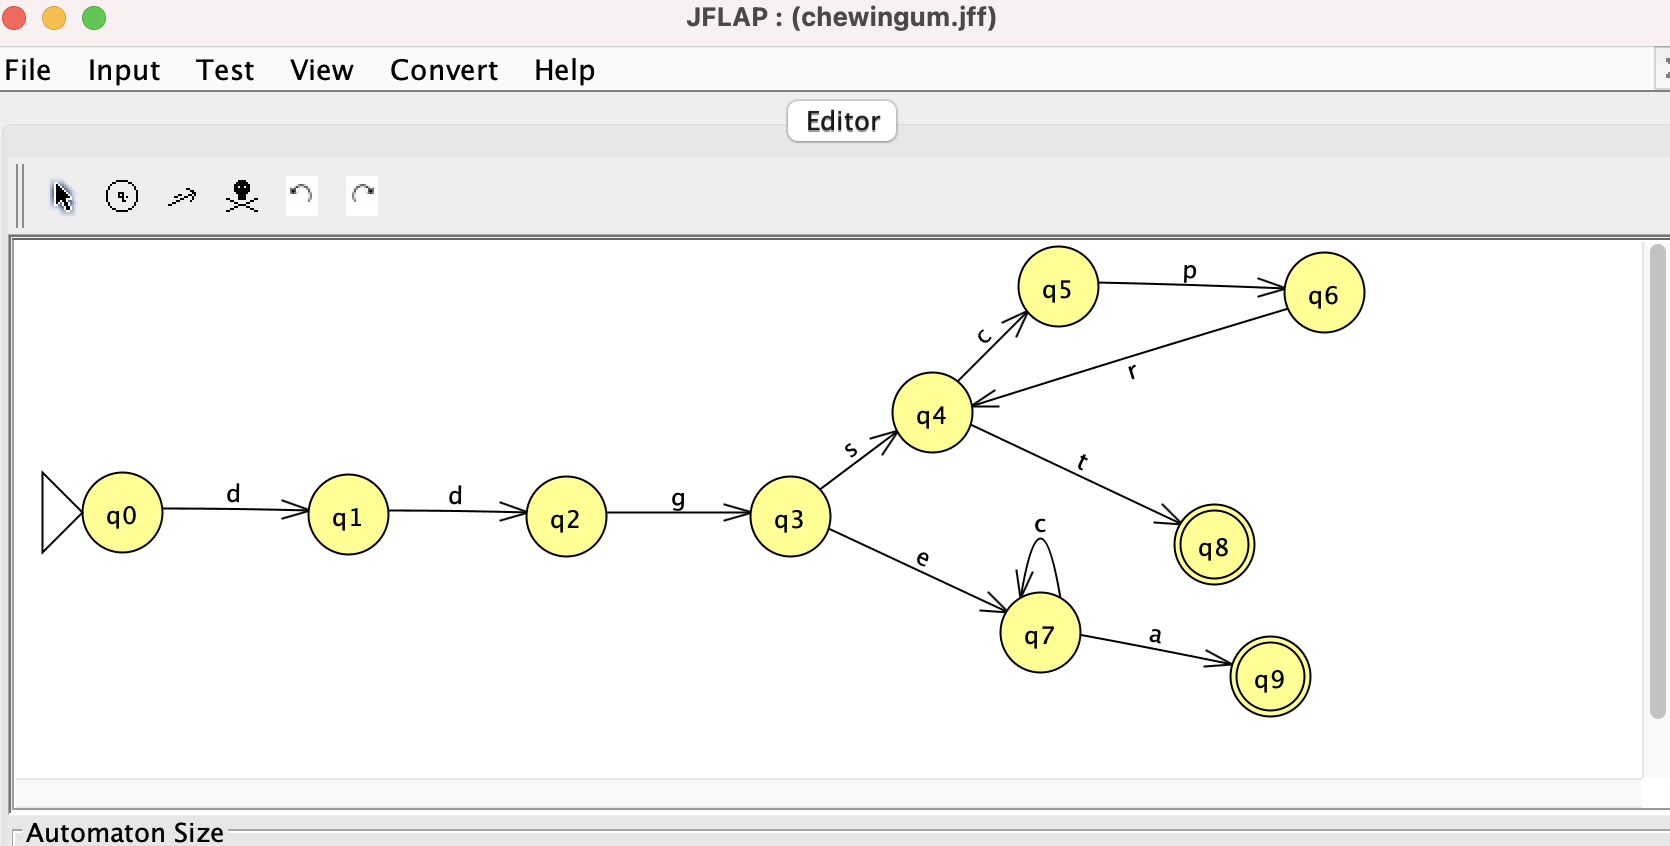
\includegraphics[scale=0.4]{Figures/chewing_gum_automaton.png}
  \end{center}

\end{frame}



%-------------------------------------------------------------
\begin{frame}[fragile]\frametitle{Recap: Classical Finite-State Automata}
  
  \blue{Central ingredients:}
  \begin{itemize}
  \item States (circles)
  \item Transitions (arcs between states) annotated with symbols of an alphabet
  \item One \emph{initial} state, marked with triangle (where execution starts)
  \item One or several \emph{final} states, marked by double circle (where execution ends)
  \end{itemize}


  \blue{Central notions:}
  \begin{itemize}
  \item Symbols of an alphabet represent possible \emph{actions}
  \item Accepted \emph{word} of an automaton: sequence of symbols leading from initial to final state
    \begin{itemize}
    \item \emph{Ex.:}  \texttt{ddgscprcprt} is accepted
    \item \emph{Ex.:} \texttt{dget} is not accepted
    \end{itemize}
    The set of accepted words of an automaton make up the \emph{language} recognized by the automaton. 
  \end{itemize}

\end{frame}


%-------------------------------------------------------------
\begin{frame}[fragile]\frametitle{Towards Timed Automata}

  \blue{What remains:} Notion of \emph{discrete state}\\
    not appropriate for \emph{continuous} events (\emph{e.g.} ball rolling down a slope)


  \blue{What remains:} Two kinds of transitions:
  \begin{itemize}
  \item Action transition (inducing state change)
  \item Delay transition (inducing progression of time)
  \end{itemize}
  
\end{frame}




%======================================================================
\section{Timed Automata in Baby L4}


%======================================================================
\section{Translating to Timed Automata}






%-------------------------------------------------------------
\begin{frame}[fragile]\frametitle{Satisfiability}


The \blue{satisfiability} problem aims at determining whether a formula is
satisfiable.

\emph{Reminder:}
\begin{itemize}
\item A formula is \blue{satisfiable} if it can be made true under \emph{one}
  possible interpretation: \emph{possibly true}
\item (It is  \blue{unsatisfiable} if it can not.)
\item A formula is \blue{valid} if it is true under \emph{every}
  possible interpretation: \emph{necessarily true}
\end{itemize}

\vspace{3mm}
Examples:
\begin{itemize}
\item $a \AND (\NOT a \OR b)$ is satisfiable but not valid:
  \begin{itemize}
  \item true for $a \mapsto True, b \mapsto True$
  \item false for $a \mapsto False$ ($b$ indifferent)
  \end{itemize}
\item $a \OR \NOT a$ is valid  
\end{itemize}

\end{frame}

%-------------------------------------------------------------
\begin{frame}[fragile]\frametitle{Satisfiability}

  \blue{Validity} and \blue{satisfiability} are related:\\
  $F$ valid \hspace{5mm} iff \hspace{5mm} $\NOT F$ unsatisfiable

  \vspace{5mm}
  Thus: one of the notions suffices.
  \vspace{5mm}
  
  The satisfiability checking problem (SAT)
  \begin{itemize}
  \item Concerns formulas of propositional logic\\
    but not only (the notion extends to arbitrary logics)
  \item In the propositional case:
    \begin{itemize}
    \item solutions (interpretations) can be checked efficiently
      (\emph{polynomial} time)
    \item solutions can be hard to find\\
      worst-case: exponential time
    \item current \blue{SAT solvers} can typically treat problems of thousands of
      propositional variables
    \end{itemize}
  \end{itemize}

\end{frame}

%-------------------------------------------------------------
\begin{frame}[fragile]\frametitle{Satisfiability Modulo Theories (SMT)}

Typically, formulas have internal structure that pure SAT solvers cannot
handle.

\vspace{5mm}
\emph{Example:}\\
$(g(a) = g(b)) \AND (f(g(b), c) \neq f(g(a), c) \OR x = 2) \AND (\exists y:Int.\; 1 < y \AND y < x)$

has the propositional form:\\
$F_1 \AND (F_2 \OR F_3) \AND F_4$\\
which is satisfiable. Is the original formula satisfiable?

\vspace{5mm}
\blue{SMT} solvers are brokers between SAT solvers and specialized reasoners
for specific \blue{theories}.

\vspace{5mm}
In the example: uninterpreted functions and (quantified) arithmetic.


\end{frame}

%-------------------------------------------------------------
\begin{frame}[fragile]\frametitle{Satisfiability Modulo Theories (SMT)}

  \emph{Example:}\\
$(g(a) = g(b)) \AND (f(g(b), c) \neq f(g(a), c) \OR x = 2) \AND (\exists y:Int.\; 1 < y \AND y < x)$

\begin{enumerate}
\item Project \emph{uninterpreted function} subformulas:\\
  $(g(a) = g(b))$,  $f(g(b), c) \neq f(g(a), c)$
\item Propagate information: Under condition $(g(a) = g(b))$:\\
  $f(g(b), c) \neq f(g(a), c) \; \leadsto \; f(g(b), c) \neq f(g(b), c) \;
  \leadsto \; False$
\item Send information to SAT solver and propagate info:\\
  $(g(a) = g(b)) \AND (False \OR x = 2) \AND (\exists y:Int.\; 1 < y \AND y < x)$ $\leadsto$\\
  $(g(a) = g(b)) \AND (x = 2) \AND (\exists y:Int.\; 1 < y \AND y < x)$ 
\item Project \emph{quantified arithmetic} subformulas:\\
  $(x = 2)$, $\exists y:Int.\; 1 < y \AND y < x$
\item Propagate information: Under condition $x = 2$:\\
  $\exists y:Int.\; 1 < y \AND y < x$ \hspace{3mm} $\leadsto$ \hspace{3mm}
  $\exists y:Int.\; 1 < y \AND y < 2$ \hspace{3mm} $\leadsto$ \hspace{3mm} $False$
\item Send information to SAT solver and propagate info:\\
  $(g(a) = g(b)) \AND (x = 2) \AND False$ \hspace{3mm} $\leadsto$ \hspace{3mm} $False$
\end{enumerate}
Formula not satisfiable

\end{frame}

%-------------------------------------------------------------
\begin{frame}[fragile]\frametitle{Satisfiability Modulo Theories (SMT)}

  Results may depend on the \blue{mathematical theory} under consideration:

  \emph{Example:}
  \begin{itemize}
  \item $(\exists y:\textbf{Int}.\; 1 < y \AND y < 2) \; \leadsto \; False$
  \item $(\exists y:\textbf{Real}.\; 1 < y \AND y < 2) \; \leadsto \; True$
  \item $(\exists y:\textbf{Real}.\; 1 < y \AND y < 1 + \epsilon) \; \leadsto \; True$
  \item $(\exists y:\textbf{Float}.\; 1 < y \AND y < 1 + \epsilon) \; \leadsto \; ???$
  \end{itemize}

  \vspace{5mm}
Specific reasoners have specialized capabilities:
\begin{itemize}
\item Uninterpreted function symbols:
  $f(x, 3) = f(3, y)$ cannot be simplified further
\item In arithmetics:\\
    $x + 3 = 3 + y$ $\; \leadsto \;$ [commutativity]\\
    $x + 3 = y + 3$ $\; \leadsto \;$ [cancellation]\\
    $x = y$
\end{itemize}
  
\end{frame}

%-------------------------------------------------------------
\begin{frame}[fragile]\frametitle{Mathematical theory}

  A mathematical theory is a signature (set of function and predicate symbols)
  with associated properties.

  \emph{Example:} Theory of Arrays (SMT Lib standard p. 39):

\small
\begin{verbatim}
(theory ArraysEx
:sorts ( (Array 2) )
:funs ((par (X Y) (select (Array X Y) X Y))
       (par (X Y) (store (Array X Y) X Y (Array X Y))) )
:definition
" - (forall ((a (Array s1 s2)) (i s1) (e s2))
       (= (select (store a i e) i) e))
  - (forall ((a (Array s1 s2)) (i s1) (j s1) (e s2))
     (=> (distinct i j) 
         (= (select (store a i e) j) (select a j))))
  - (forall ((a (Array s1 s2)) (b (Array s1 s2)))
     (=>
      (forall ((i s1)) (= (select a i) (select b i))) 
      (= a b))) "
)
\end{verbatim}
\normalsize  

\end{frame}

%-------------------------------------------------------------
\begin{frame}[fragile]\frametitle{Mathematical theory}

  \begin{itemize}
  \item QF for the restriction to quantifier free formulas
  \item  A or AX for the theory ArraysEx
  \item     BV for the theory FixedSizeBitVectors
  \item     FP (forthcoming) for the theory FloatingPoint
  \item     IA for the theory Ints (Integer Arithmetic)
  \item     RA for the theory Reals (Real Arithmetic)
  \item     IRA for the theory Reals-Ints (mixed Integer Real Arithmetic)
  \item     IDL for Integer Difference Logic
  \item     RDL for Rational Difference Logic
  \item     L before IA, RA, or IRA for the linear fragment of those
    arithmetics
  \item     N before IA, RA, or IRA for the non-linear fragment of those
    arithmetics
  \item     UF for the extension allowing free sort and function symbols
  \end{itemize}
  
\end{frame}

%-------------------------------------------------------------
\begin{frame}[fragile]\frametitle{Theories and their interaction}
  see \url{http://smtlib.cs.uiowa.edu/logics.shtml}


\end{frame}




%======================================================================
\section{SMT-LIB: Interacting with an SMT solver}


%-------------------------------------------------------------
\begin{frame}[fragile]\frametitle{SMT solvers}

  Several solvers support these logics to varying degrees:

  \begin{itemize}
  \item Z3 (*) \url{https://github.com/Z3Prover/z3/wiki}
  \item CVC4 (*) \url{https://cvc4.github.io/}\\
    with CVC5 \url{https://cvc5.github.io/} under development
  \item Boolector \url{https://github.com/Boolector}\\
    specialized on byte arrays
  \item Yices \url{https://yices.csl.sri.com/} (PVS)
  \item Alt-Ergo \url{https://ocamlpro.github.io/alt-ergo/} (Frama-C)
  \item Mathsat (*) \url{https://mathsat.fbk.eu/}
  \end{itemize}

(*): works at least partly with L4
\end{frame}


%-------------------------------------------------------------
\begin{frame}[fragile]\frametitle{SMT-LIB}

  SMT-LIB is:
  \begin{itemize}
  \item a standardized common input format for describing proof problems
  \item a partly standardized output format for retrieving proof results
  \item a protocol for interacting with solvers
  \end{itemize}

  Purpose: 
  \begin{itemize}
  \item Make SMT solvers more easily accessible to third-party tools
  \item Facilitate benchmarking / contests
  \end{itemize}
\end{frame}


%-------------------------------------------------------------
\begin{frame}[fragile]\frametitle{SMT Input file}

  \blue{Declarations of sorts and constants / predicates}
\begin{verbatim}
(set-option :print-success true )
(set-option :produce-models true )
(set-logic LIA )
(declare-sort Class 0 )
(declare-sort Animal 0 )
(declare-sort Cat 0 )
(declare-sort Mouse 0 )
(declare-fun isCat (Animal ) Bool )
(declare-fun isMouse (Animal ) Bool )
(declare-fun Age (Animal Int ) Bool )
(declare-fun garfield () Animal )
(declare-fun mickey () Animal )
\end{verbatim}
\end{frame}

  
%-------------------------------------------------------------
\begin{frame}[fragile]\frametitle{SMT Input file}

\blue{ Formula to be proved and call of checker}
\begin{verbatim}
(assert 
(and (and (Age garfield 3 ) (Age mickey 2 ) ) 
(and (forall ((a Animal ) ) 
   (=> true (not (and (isCat a ) (isMouse a ) ) ) ) ) 
   (and (=> true (isCat garfield ) ) 
   (and (=> true (isMouse mickey ) ) (forall ((c Animal ) ) 
   (forall ((m Animal ) ) (forall ((ac Int ) ) 
   (forall ((am Int ) ) 
   (=> (and (isCat c ) (and (isMouse m ) 
         (and (Age c ac )
         (and (>= ac 5 ) (Age m am ) ) ) ) ) 
       (< am 1 ) ) ) ) ) ) ) ) ) ) )
(check-sat )
\end{verbatim}

\end{frame}

%-------------------------------------------------------------
\begin{frame}[fragile]\frametitle{SMT Output file}

  \blue{Generated model} (not meant to be readable)
  \small
  \begin{verbatim}
(model 
(declare-fun Animal!val!1 () Animal ) 
(declare-fun Animal!val!0 () Animal ) 
(define-fun garfield () Animal Animal!val!0 ) 
(define-fun mickey () Animal Animal!val!1 ) 
(define-fun isMouse ((x!0 Animal ) ) Bool 
  (= (ite(= x!0 Animal!val!0 ) Animal!val!0 Animal!val!1) 
     Animal!val!1)) 

(define-fun isCat ((x!0 Animal ) ) Bool 
   (= (ite (= x!0 Animal!val!0 ) Animal!val!0 Animal!val!1)
   Animal!val!0 ) ) 

(define-fun Age ((x!0 Animal ) (x!1 Int ) ) Bool  ... ) )

\end{verbatim}  
\normalsize
\end{frame}


%======================================================================
\section{L4 and SMT}

%-------------------------------------------------------------
\begin{frame}[fragile]\frametitle{Proving statements in L4}

  \begin{itemize}
  \item \texttt{assert} statements in L4 can lead to SMT prover calls
  \item \dots{} using information some or parts of the facts / rules of a spec
  \end{itemize}


  \vspace{5mm}
  \blue{ What is checked, based on which information?}
  \vspace{5mm}
  
  Can in part be configured with \emph{instructions} accompanying
  \texttt{assert} (and in the future: \texttt{rule}) statements.

\end{frame}


%-------------------------------------------------------------
\begin{frame}[fragile]\frametitle{Configuring the reasoner}

\begin{verbatim}
assert {SMT: {...},
        sCASP: {...},
        foobar: {...}
       }
Goal
\end{verbatim}

  \begin{itemize}
  \item All the registered reasoners will be invoked on the \texttt{Goal}
    (see below).
  \item Inexistent reasoners will be ignored
  \end{itemize}

\end{frame}


%-------------------------------------------------------------
\begin{frame}[fragile]\frametitle{What will be proved?}

  \blue{Prerequisites:} Each rule gives rise to a formula

  \emph{Example:}

\begin{alltt}  
  \textbf{rule} <R>
  \textbf{for} x : Integer
  \textbf{if} P(x)
  \textbf{then} Q(x)
\end{alltt}
generates the formula $\forall x: Integer.\; P(x) \IMPL Q(X)$

\vspace{3mm}

There is an \blue{active ruleset} $R_1, \dots,  R_n$ (configurable, see below).

\begin{itemize}
\item 
\begin{verbatim}
assert {SMT: {consistent, ...} }  Goal
\end{verbatim}
checks if $R_1 \AND \dots \AND R_n \AND Goal$ is \emph{satisfiable}

\item 
\begin{verbatim}
assert {SMT: {valid, ...} } Goal
\end{verbatim}
checks if $R_1 \AND \dots \AND R_n \IMPL Goal$ is \emph{valid}\\
(corresponds to: $R_1 \AND \dots \AND R_n \AND \NOT Goal$ unsatisfiable)
  
\end{itemize}

\end{frame}


%-------------------------------------------------------------
\begin{frame}[fragile]\frametitle{Which formulas are taken into
    consideration?}

  \blue{Prerequisites:} a \emph{default rule set}:
  \begin{itemize}
  \item currently the set of all rules of the spec
  \item to be reconsidered \dots
  \end{itemize}
  
  
The \blue{active ruleset} is configurable by the \texttt{rules} section:
\begin{verbatim}
assert {SMT: { rules: {rulespec}, ...} }
Goal
\end{verbatim}

where the \emph{rulespec} is a combination of:
  \begin{itemize}
  \item \verb|only: {list of rules}|: only take these rules
  \item \verb|del:  {list of rules}|: rules to be removed from ruleset
  \item \verb|add:  {list of rules}|: rules to be added to ruleset after
    removing the \texttt{del}-rules (currently not useful)
  \end{itemize}

\end{frame}


%-------------------------------------------------------------
\begin{frame}[fragile]\frametitle{How to configure the solver?}

Configure the solver with the \texttt{config} clause
\begin{verbatim}
assert {SMT: { config: {solver: z3, 
                        logic: LIA, 
                        loglevel: 0}, ...} }
Goal
\end{verbatim}

\begin{itemize}
\item Solver:
  \begin{itemize}
  \item Has to be installed in advance, executable on execution path
  \item Cannot be done on the fly (invocation parameters hard-wired)
  \item Currently, only \texttt{z4}, \texttt{cvc3}, \texttt{mathsat} are configured
  \end{itemize}
\item Logic: Any of the SMT-LIB logics. 
\item \texttt{loglevel}: Level of verbosity for tracing interaction with SMT solver
\end{itemize}

\end{frame}


%-------------------------------------------------------------
\begin{frame}[fragile]\frametitle{L4 example model}

  \blue{Declarations}

  \begin{verbatim}
class Animal
class Cat extends Animal
class Mouse extends Animal

decl isCat: Animal -> Boolean
decl isMouse: Animal -> Boolean

decl Age : Animal -> Integer -> Boolean

decl garfield: Animal
decl mickey: Animal
\end{verbatim}
  
\end{frame}


%-------------------------------------------------------------
\begin{frame}[fragile]\frametitle{L4 example model}

  \blue{Facts}

\begin{verbatim}
fact <CatNotMouse>
for a: Animal
not (isCat a && isMouse a)

fact <GarfieldCat>
isCat garfield

fact <MickeyMouse>
isMouse mickey
\end{verbatim}
  
\end{frame}


%-------------------------------------------------------------
\begin{frame}[fragile]\frametitle{L4 example model}

  \blue{Main rule and assertions}

\begin{verbatim}
# no mice older than 1 year have a chance to survive 
# being chased by cats older than 5 years
rule <OldCatsChaseWell>
for c: Animal, m: Animal, ac: Integer, am: Integer
if isCat c && isMouse m && Age c ac 
   && ac >= 5 && Age m am 
then am < 1

# inconsistent, proof fails
assert {SMT: {consistent}}
Age garfield 5  && Age mickey 2

# consistent, model found
assert {SMT: {consistent}} 
Age garfield 3 && Age mickey 2

\end{verbatim}

\end{frame}



%-------------------------------------------------------------
\begin{frame}[fragile]\frametitle{L4 example model}

  \blue{Run checker:}
\texttt{stack run -- l4 smt l4/garfield.l4}

\begin{itemize}
\item First formula: \texttt{Formula unsatisfiable.}
\item Second formula:
\begin{verbatim}
Formula satisfiable, found model.
Predicates: 
isMouse mickey = true
isCat garfield = true
Age mickey intArg1 = 
   (and (<= 2 intArg1) (not (<= 3 intArg1)))
Age garfield intArg1 = 
  (and (<= 2 intArg1) 
  (and (<= 3 intArg1) (not (<= 5 intArg1))))
Remaining predicates: false
\end{verbatim}
\end{itemize}

\end{frame}

%-------------------------------------------------------------

\end{document}


%%% Local Variables: 
%%% mode: latex
%%% TeX-master: t
%%% coding: utf-8
%%% End: 
